\documentclass{article}

%%%%%%%%%%%%%%%%%%%%%%%%%%%%%%%%%%%%%%%%%
% Lachaise Assignment
% Structure Specification File
% Version 1.0 (26/6/2018)
%
% This template originates from:
% http://www.LaTeXTemplates.com
%
% Authors:
% Marion Lachaise & François Févotte
% Vel (vel@LaTeXTemplates.com)
%
% License:
% CC BY-NC-SA 3.0 (http://creativecommons.org/licenses/by-nc-sa/3.0/)
% 
%%%%%%%%%%%%%%%%%%%%%%%%%%%%%%%%%%%%%%%%%

%----------------------------------------------------------------------------------------
%	PACKAGES AND OTHER DOCUMENT CONFIGURATIONS
%----------------------------------------------------------------------------------------

\usepackage{amsmath,amsfonts,stmaryrd,amssymb} % Math packages

\usepackage{enumerate} % Custom item numbers for enumerations

\usepackage[ruled]{algorithm2e} % Algorithms

\usepackage[framemethod=tikz]{mdframed} % Allows defining custom boxed/framed environments

\usepackage{listings} % File listings, with syntax highlighting
\lstset{
	basicstyle=\ttfamily, % Typeset listings in monospace font
}

%----------------------------------------------------------------------------------------
%	DOCUMENT MARGINS
%----------------------------------------------------------------------------------------

\usepackage{geometry} % Required for adjusting page dimensions and margins

\geometry{
	paper=a4paper, % Paper size, change to letterpaper for US letter size
	top=2.5cm, % Top margin
	bottom=3cm, % Bottom margin
	left=2.5cm, % Left margin
	right=2.5cm, % Right margin
	headheight=14pt, % Header height
	footskip=1.5cm, % Space from the bottom margin to the baseline of the footer
	headsep=1.2cm, % Space from the top margin to the baseline of the header
	%showframe, % Uncomment to show how the type block is set on the page
}

%----------------------------------------------------------------------------------------
%	FONTS
%----------------------------------------------------------------------------------------

\usepackage[utf8]{inputenc} % Required for inputting international characters
\usepackage[T1]{fontenc} % Output font encoding for international characters

\usepackage{XCharter} % Use the XCharter fonts

%----------------------------------------------------------------------------------------
%	COMMAND LINE ENVIRONMENT
%----------------------------------------------------------------------------------------

% Usage:
% \begin{commandline}
%	\begin{verbatim}
%		$ ls
%		
%		Applications	Desktop	...
%	\end{verbatim}
% \end{commandline}

\mdfdefinestyle{commandline}{
	leftmargin=10pt,
	rightmargin=10pt,
	innerleftmargin=15pt,
	middlelinecolor=black!50!white,
	middlelinewidth=2pt,
	frametitlerule=false,
	backgroundcolor=black!5!white,
	frametitle={Command Line},
	frametitlefont={\normalfont\sffamily\color{white}\hspace{-1em}},
	frametitlebackgroundcolor=black!50!white,
	nobreak,
}

% Define a custom environment for command-line snapshots
\newenvironment{commandline}{
	\medskip
	\begin{mdframed}[style=commandline]
}{
	\end{mdframed}
	\medskip
}

%----------------------------------------------------------------------------------------
%	FILE CONTENTS ENVIRONMENT
%----------------------------------------------------------------------------------------

% Usage:
% \begin{file}[optional filename, defaults to "File"]
%	File contents, for example, with a listings environment
% \end{file}

\mdfdefinestyle{file}{
	innertopmargin=1.6\baselineskip,
	innerbottommargin=0.8\baselineskip,
	topline=false, bottomline=false,
	leftline=false, rightline=false,
	leftmargin=2cm,
	rightmargin=2cm,
	singleextra={%
		\draw[fill=black!10!white](P)++(0,-1.2em)rectangle(P-|O);
		\node[anchor=north west]
		at(P-|O){\ttfamily\mdfilename};
		%
		\def\l{3em}
		\draw(O-|P)++(-\l,0)--++(\l,\l)--(P)--(P-|O)--(O)--cycle;
		\draw(O-|P)++(-\l,0)--++(0,\l)--++(\l,0);
	},
	nobreak,
}

% Define a custom environment for file contents
\newenvironment{file}[1][File]{ % Set the default filename to "File"
	\medskip
	\newcommand{\mdfilename}{#1}
	\begin{mdframed}[style=file]
}{
	\end{mdframed}
	\medskip
}

%----------------------------------------------------------------------------------------
%	NUMBERED QUESTIONS ENVIRONMENT
%----------------------------------------------------------------------------------------

% Usage:
% \begin{question}[optional title]
%	Question contents
% \end{question}

\mdfdefinestyle{question}{
	innertopmargin=1.2\baselineskip,
	innerbottommargin=0.8\baselineskip,
	roundcorner=5pt,
	nobreak,
	singleextra={%
		\draw(P-|O)node[xshift=1em,anchor=west,fill=white,draw,rounded corners=5pt]{%
		Question \theQuestion\questionTitle};
	},
}

\newcounter{Question} % Stores the current question number that gets iterated with each new question

% Define a custom environment for numbered questions
\newenvironment{question}[1][\unskip]{
	\bigskip
	\stepcounter{Question}
	\newcommand{\questionTitle}{~#1}
	\begin{mdframed}[style=question]
}{
	\end{mdframed}
	\medskip
}

%----------------------------------------------------------------------------------------
%	WARNING TEXT ENVIRONMENT
%----------------------------------------------------------------------------------------

% Usage:
% \begin{warn}[optional title, defaults to "Warning:"]
%	Contents
% \end{warn}

\mdfdefinestyle{warning}{
	topline=false, bottomline=false,
	leftline=false, rightline=false,
	nobreak,
	singleextra={%
		\draw(P-|O)++(-0.5em,0)node(tmp1){};
		\draw(P-|O)++(0.5em,0)node(tmp2){};
		\fill[black,rotate around={45:(P-|O)}](tmp1)rectangle(tmp2);
		\node at(P-|O){\color{white}\scriptsize\bf !};
		\draw[very thick](P-|O)++(0,-1em)--(O);%--(O-|P);
	}
}

% Define a custom environment for warning text
\newenvironment{warn}[1][Warning:]{ % Set the default warning to "Warning:"
	\medskip
	\begin{mdframed}[style=warning]
		\noindent{\textbf{#1}}
}{
	\end{mdframed}
}

%----------------------------------------------------------------------------------------
%	INFORMATION ENVIRONMENT
%----------------------------------------------------------------------------------------

% Usage:
% \begin{info}[optional title, defaults to "Info:"]
% 	contents
% 	\end{info}

\mdfdefinestyle{info}{%
	topline=false, bottomline=false,
	leftline=false, rightline=false,
	nobreak,
	singleextra={%
		\fill[black](P-|O)circle[radius=0.4em];
		\node at(P-|O){\color{white}\scriptsize\bf i};
		\draw[very thick](P-|O)++(0,-0.8em)--(O);%--(O-|P);
	}
}

% Define a custom environment for information
\newenvironment{info}[1][Info:]{ % Set the default title to "Info:"
	\medskip
	\begin{mdframed}[style=info]
		\noindent{\textbf{#1}}
}{
	\end{mdframed}
}
 % Include the file specifying the document structure and custom commands

\usepackage{graphicx}
\usepackage{float}
\usepackage{caption}
\usepackage{parskip}
\usepackage{hyperref}
\renewcommand{\thealgocf}{} % Stop numbering in header of algorithms
\SetKwRepeat{Do}{do}{while} % Do while loop for algorithms

%----------------------------------------------------------------------------------------
%	ASSIGNMENT INFORMATION
%----------------------------------------------------------------------------------------

\title{EELE465 NCUR REPORT:\\ Creating a Simple Wireless Tor Access Point}

\author{Ryan French\\ \texttt{ryanfrench3@montana.edu}\\ \texttt{Graduate Student, Department of Physics}\\ \texttt{Montana State Physics University - \today}}

\date{}
%----------------------------------------------------------------------------------------

\begin{document}
\maketitle % Print the title

%\begin{info} % Information block
%	This is an interesting piece of information, to which the reader should pay special attention. Fusce varius orci ac magna dapibus porttitor. In tempor leo a neque bibendum sollicitudin. Nulla pretium fermentum nisi, eget sodales magna facilisis eu. Praesent aliquet nulla ut bibendum lacinia. Donec vel mauris vulputate, commodo ligula ut, egestas orci. Suspendisse commodo odio sed hendrerit lobortis. Donec finibus eros erat, vel ornare enim mattis et.
%\end{info}
%----------------------------------------------------------------------------------------


%----------------------------------------------------------------------------------------
%	                            INTRODUCTION
%----------------------------------------------------------------------------------------

\section*{Introduction}

In today's ever-increasing surveillance of internet activity, people are rightly becoming more vigilant of their internet footprint. The two most popular solutions sold to consumers are:

\begin{enumerate}
\item Proxies
\begin{itemize}
\item The least secure method of anonymity. The client's requests are passed through an intermediary server, which masks the client's IP address.
\end{itemize}
\item Virtual Private Networks (VPN)
\begin{itemize}
\item Very secure. A client's requests are sent to a dedicated server through an encrypted tunnel.
\end{itemize}
\end{enumerate}

There are issues with both of these methods, however. Most notably is that personal information is being stored on the servers, which is something that cannot be tolerated in some contexts.

For those who require more anonymity, Tor is the go-to service. Tor is an decentralized network which encrypts a client's requests as it bounces between a number (usually 3) of volutary relays.\cite{Tor} This means that all of the data sent between relays is inaccessible by means of man-in-the-middle attacks or other malicious attempts to intercept data. This makes Tor the solution that is used to access the "Dark Web," the largest part of the internet, which contain sites not indexed by any ordinary web browsers. Tor is not a perfect solution, however, and additional measures must be implemented to confidently lock down the client's identity.

Though Tor is usually thought of as a browser, it is a more fundamental anonymizing software. Because of this, it is possible to build a wireless access point (WAP) that filters the client's requests through the Tor network. Constructing one of these access points only requires a wireless chipset and a microcontroller as its main components. An excellent example of this setup is the Arduino Yún.\cite{ArduinoYun} From here on, all explanations will reference this board, though it's possible to use any microcontroller and wireless chipset.


%----------------------------------------------------------------------------------------

% Numbered question, with subquestions in an enumerate environment
%\begin{question}
%	Quisque ullamcorper placerat ipsum. Cras nibh. Morbi vel justo vitae lacus tincidunt ultrices. Lorem ipsum dolor sit amet, consectetuer adipiscing elit.
%
%	% Subquestions numbered with letters
%	\begin{enumerate}[(a)]
%		\item Do this.
%		\item Do that.
%		\item Do something else.
%	\end{enumerate}
%\end{question}
%
%------------------------------------------------


%----------------------------------------------------------------------------------------
%                         IMPLEMENTATION
%----------------------------------------------------------------------------------------

\section*{Implementation}
\subsection*{Microcontroller Side: Access Point}

Wireless chipsets usually contain a specialized version of the Linux operating system called OpenWrt. It is this OS that will control the wireless connections. However, this chipset is only designed to handle its own connections, which means that it is necessary to obtain another wireless chipset. A popular chipset is the ESP8266, which can easily be obtained in modular form. This connection will be handled explicitly by the microcontroller.

Setting up the access point is relatively easy. The process works as follows:

\begin{enumerate}
\item The ESP8266 scans for incoming traffic. Once detected, it passes the information to the MCU.
\item The MCU interprets the data. It is at this point that the MCU can spoof information in the incoming packets if additional anonymity is wanted.
\item The MCU sends this information to the on-board wireless chipset through a bridge.
\item This chipset runs the packets through the Tor process to forward the request.
\item The request is processed and sent back through this chain, and the ESP8266 returns the requested data to the client.
\end{enumerate}

Of course, this explanation is very simplified, as configuring the wireless communication and bridges involves modifying plenty of configuration files. It's also important to test the Tor connection to make sure that the client's information (IP address, MAC address) isn't being leaked. See the "Client Side" subsection for more information on this.

The MCU on the WAP can handle plenty of things in addition to providing a bridge between the wireless chipsets. An excellent example of this is using the MCU to control several LEDs indicating the status of the connections. For example, one set of LEDs can confirm successful connection to the Tor network, another set can confirm that the client is sending requests to secure servers (i.e., servers with HTTPS).

% \begin{center}
% 	\begin{minipage}{0.6\linewidth} % Adjust the minipage width to accomodate for the length of algorithm lines
% 		\begin{algorithm}[H]
% %			\KwIn{$(N, DEC)$:  Number of Loops, Decrement Initial Value}  % Algorithm inputs
% 			%\KwResult{$(c, d)$, such that $a+b = c + d$} % Algorithm outputs/results
% 			\medskip
% 			Clear Column Pins\;
% 			\For {column pins}{
% 			Set Column Pin\;
% 			\For {row pins}{
% 			Read Pin\;
% 			\If {read pin}{
% 			add\_button\_press()\;
% 			}
% 			}
% 			Clear Column Pin\;
% 			}
% 			Set Column Pins\;
% 			Send I2C data\;
% 			\caption{Read Key Press} % Algorithm name
% 			\label{alg:KeyPress}   % optional label to refer to
% 		\end{algorithm}
% 	\end{minipage}
% \end{center}


\subsection*{Client Side}

The client side has several responsibilities to maintain anonymity. Above, it was mentioned that it is important to confirm that the client's information isn't being leaked somehow. There are three major things that the client must do to protect against this:

\begin{enumerate}
\item MAC spoofing. A MAC address is an identifier that is tied to each individual network interface controller. Though Tor usually handles this, it is an additional layer of security to spoof it before handing off information to the access point.
\item DNS setup. A DNS is a system that maps domain names to IP addresses. For example, the DNS will translate the request "www.google.com" to its corresponding IP address before forwarding the request. Without configuring a custom DNS, requests are sent to the client's Internet Service Provider's DNS, which stores information about the client and its requests.
\item IP address spoofing. This is handled by Tor, but it is the client's repsonsibility to confirm that this is happening.
\end{enumerate}

There exist many ways for a client to confirm that all of the above are satisfied. The easiest is to request data from specialized web servers that return as much information about the client as possible. In fact, in this case, the MCU can handle this through its bridge to the on-board chipset, which simplifies the responsibilities of the client.

%----------------------------------------------------------------------------------------

%% Numbered question, with an optional title
%\begin{question}[\itshape (with optional title)]
%
%\end{question}


%----------------------------------------------------------------------------------------
%					CONCLUSION
%----------------------------------------------------------------------------------------
\section*{Conclusion}

Though many consumers are decently anonymized through commercialized solutions like proxies and VPNs, these methods can fall short. The Tor network, when used properly, is a much better solution for clients who require more than what these other solutions provide. Because the setup of Tor is relatively easy, it is possible to create a small wireless access point that filters all traffic through Tor. This is a great solution for avoiding most nefarious attempts to gather information about a client.


\section*{Note}

Information security has been a hobby of mine on-and-off for about 7 months. I have familiarity with many of the topics I've presented here, however, I am by no means an authority. There may be some minor mistakes in interpretation. I must also note that I only advise using Tor for informational purposes, and by no means do I encourage using it with dangerous or illicit intent.




%----------------------------------------------------------------------------------------


%\section{Extra nonsense}
%
%% File contents
%\begin{file}[hello.py]
%\begin{lstlisting}[language=Python]
%#! /usr/bin/python
%
%import sys
%sys.stdout.write("Hello World!\n")
%\end{lstlisting}
%\end{file}

%----------------------------------------------------------------------------------------

%% Command-line "screenshot"
%\begin{commandline}
%	\begin{verbatim}
%		$ chmod +x hello.py
%		$ ./hello.py
%
%		Hello World!
%	\end{verbatim}
%\end{commandline}

%% Warning text, with a custom title
%\begin{warn}[Notice:]
%  In congue risus leo, in gravida enim viverra id. Donec eros mauris, bibendum vel dui at, tempor commodo augue. In vel lobortis lacus. Nam ornare ullamcorper mauris vel molestie. Maecenas vehicula ornare turpis, vitae fringilla orci consectetur vel. Nam pulvinar justo nec neque egestas tristique. Donec ac dolor at libero congue varius sed vitae lectus. Donec et tristique nulla, sit amet scelerisque orci. Maecenas a vestibulum lectus, vitae gravida nulla. Proin eget volutpat orci. Morbi eu aliquet turpis. Vivamus molestie urna quis tempor tristique. Proin hendrerit sem nec tempor sollicitudin.
%\end{warn}

\pagebreak

%\section*{Appendix}
%
%\begin{centering}
%\begin{figure}[H]
%%\label{fig:Flowchart}
%\centering
%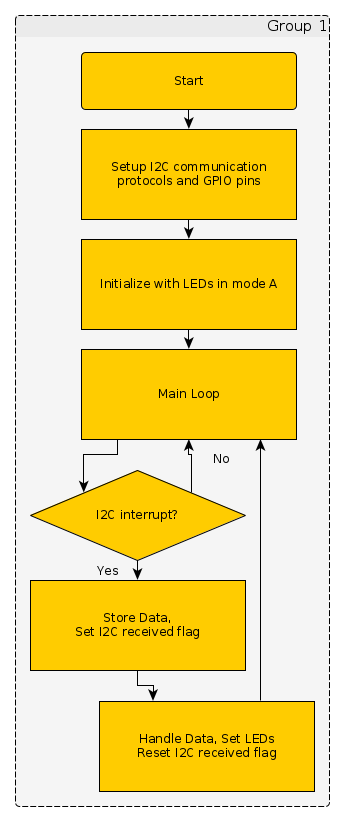
\includegraphics[width = 0.6\textwidth]{flowchart.png}
%\captionsetup{format = hang, width = 0.75\textwidth}
%\caption{MSP430FR2310's code}
%\label{fig:Flowchart}
%\end{figure}
%\end{centering}

\pagebreak

%\begin{centering}
%\begin{figure}[H]
%\label{system}
%\centering
%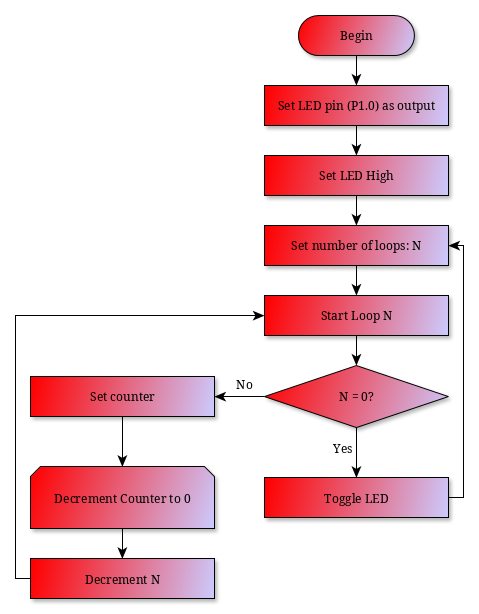
\includegraphics[width = 0.6\textwidth]{Lab0_part2.png}
%\captionsetup{format = hang, width = 0.75\textwidth}
%\caption{Timer Interrupt Solution}
%\label{fig:Int}
%\end{figure}
%\end{centering}
%
%\pagebreak
%
%\begin{centering}
%\begin{figure}[H]
%\label{system}
%\centering
%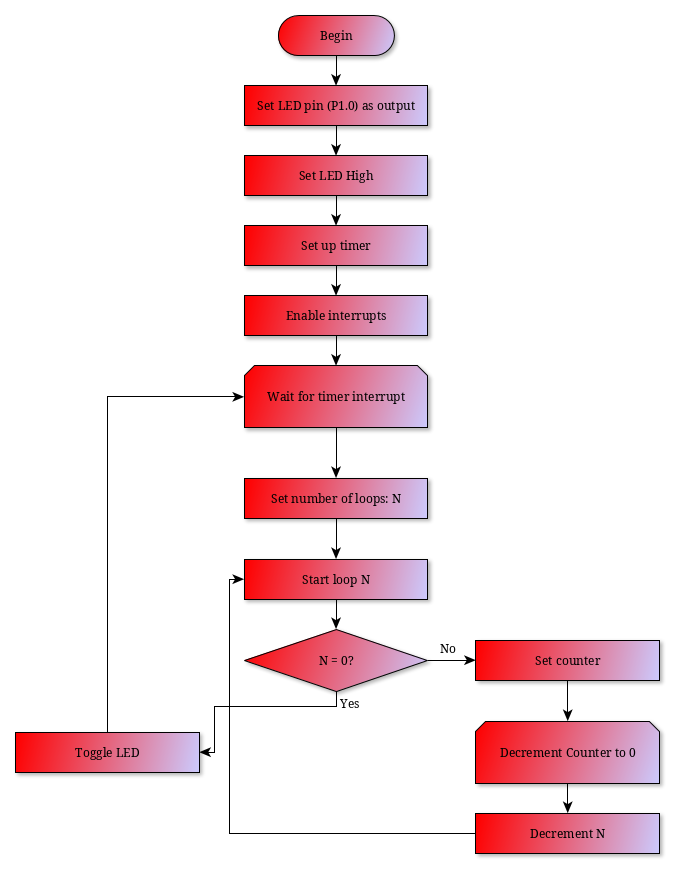
\includegraphics[width = 0.75\textwidth]{Lab0_part3.png}
%\captionsetup{format = hang, width = 0.75\textwidth}
%\caption{Combined Solution}
%\label{fig:DecInt}
%\end{figure}
%\end{centering}


\bibliography{refs}
\bibliographystyle{ieeetr}



%----------------------------------------------------------------------------------------
%	END OF DOCUMENT
%----------------------------------------------------------------------------------------

\end{document}
